\documentclass{article}
\usepackage[utf8]{inputenc}
\usepackage[T1]{fontenc}
\usepackage{hyperref}
\usepackage{url}
\usepackage{booktabs}
\usepackage{amsfonts,amsmath,amssymb,amsthm}
\usepackage{graphicx}
\usepackage{xcolor}
\usepackage{subcaption}
% Standard margins for JMLR-length paper
\usepackage[margin=1in]{geometry}

% Theorem environments
\newtheorem{theorem}{Theorem}
\newtheorem{lemma}[theorem]{Lemma}
\newtheorem{corollary}[theorem]{Corollary}
\newtheorem{definition}[theorem]{Definition}
\newtheorem{proposition}[theorem]{Proposition}
\newtheorem{remark}[theorem]{Remark}
\newtheorem{axiom}{Axiom}

% Commands
\newcommand{\R}{\mathbb{R}}
\newcommand{\E}{\mathbb{E}}
\newcommand{\Var}{\mathrm{Var}}
\newcommand{\SHAP}{\mathrm{SHAP}}
\newcommand{\DASH}{\textsc{Dash}}
\newcommand{\GBDT}{\textsc{GBDT}}

\title{The Attribution Impossibility: Faithful, Stable, and Complete Feature Rankings Cannot Coexist Under Collinearity}

\author{
  Drake Caraker\thanks{Corresponding author: \texttt{drakecaraker@gmail.com}} \quad
  Bryan Arnold \quad
  David Rhoads \\[4pt]
  \textit{Independent Researchers}
}

\begin{document}
\maketitle
\tableofcontents
\newpage

%%%%%%%%%%%%%%%%%%%%%%%%%%%%%%%%%%%%%%%%%%%%%%%%%%%%%%%%%%%%%
%% ABSTRACT
%%%%%%%%%%%%%%%%%%%%%%%%%%%%%%%%%%%%%%%%%%%%%%%%%%%%%%%%%%%%%

\begin{abstract}
We characterize the complete attribution design space under feature collinearity: exactly two families of methods exist---faithful-complete methods (unstable, with rankings that flip up to 50\% of the time) and ensemble methods like \DASH{} (stable, reporting ties for symmetric features)---and no method lies outside this dichotomy.
The foundation is the \emph{Attribution Impossibility}: no feature ranking can be simultaneously faithful, stable, and complete when features are collinear.
The impossibility is quantitative: we derive architecture-discriminating bounds showing the attribution ratio diverges as $1/(1{-}\rho^2)$ for gradient boosting, is infinite for Lasso, and converges for random forests.
\DASH{} ensemble averaging is provably Pareto-optimal on the stable branch, achieving the Cram\'er--Rao variance bound with a tight ensemble size formula.
In a survey of 37 public datasets, approximately 60\% exhibit attribution instability (conservative lower bound: survey power 32\% at the 10\% threshold; true prevalence likely higher).
Switching to conditional SHAP does not escape the impossibility when features have equal causal effects.
The framework includes practical diagnostics---a $Z$-test workflow and single-model screening tool---and has direct consequences for fairness auditing: SHAP-based proxy discrimination audits are provably unreliable under collinearity.
The design space theorem, diagnostics, and impossibility are mechanically verified in Lean~4 (188 theorems from 15 domain-specific + 3 query-complexity axioms, 0 \texttt{sorry})---to our knowledge, the first formally verified impossibility in explainable AI.
Code and Lean proofs are available at \url{https://github.com/DrakeCaraker/dash-impossibility-lean}.
\end{abstract}

%%%%%%%%%%%%%%%%%%%%%%%%%%%%%%%%%%%%%%%%%%%%%%%%%%%%%%%%%%%%%
%% 1. INTRODUCTION
%%%%%%%%%%%%%%%%%%%%%%%%%%%%%%%%%%%%%%%%%%%%%%%%%%%%%%%%%%%%%

\section{Introduction}
\label{sec:intro}

Feature attribution methods assign importance scores to input variables, enabling practitioners to understand which features drive a model's predictions.
SHAP values \cite{lundberg2017unified} have become the dominant framework, offering a principled connection to cooperative game theory.
Yet under feature collinearity, SHAP-based rankings are unstable: retraining on bootstrap samples can invert the importance ordering of correlated features \cite{hwang2025shap}, eroding trust in explanations, complicating regulatory compliance, and producing contradictory conclusions in variable selection and causal discovery.

Several recent results have established fundamental limits on feature attribution.
\cite{bilodeau2024impossibility} prove that completeness and linearity cannot coexist; \cite{huang2024failings} show SHAP can misrank features in Boolean domains; \cite{srinivas2019full} show complete attributions cannot be weakly input-dependent; and \cite{rao2025limits} establishes Kolmogorov complexity barriers to explainability.
None of these results analyze \emph{stability}---the robustness of attributions to retraining---none provide quantitative architecture-discriminating bounds, and none offer a constructive resolution.

This paper fills these gaps.
Our main result is the \emph{Attribution Design Space Theorem} (\S\ref{sec:design-space}, Figure~\ref{fig:design-space}): a complete characterization of what is achievable when explaining models with collinear features.
The achievable set consists of exactly two families---faithful-complete methods (unstable, unfaithful to half the models) and ensemble methods like \DASH{} (stable, with within-group ties)---and \DASH{} is Pareto-optimal.
The theorem rests on an \emph{Attribution Impossibility}: for any single model trained on collinear features, faithfulness, stability, and completeness are mutually incompatible.
The impossibility has two layers.
The first is model-agnostic: formalizing the Rashomon property \cite{rudin2024amazing}, we show symmetric features are necessarily ranked in opposite orders by different near-optimal models.
The second is model-specific: we derive quantitative bounds on the attribution ratio (the factor by which the dominant feature is overweighted).
For \GBDT{}, this ratio follows $1/(1-\alpha\rho^2)$ where $\alpha$ captures the per-tree signal fraction; for Lasso it is infinite at any $\rho > 0$; for neural networks it depends on the initialization; and for random forests it is $O(1/\sqrt{T})$---converging rather than diverging.

The impossibility parallels fairness: \cite{chouldechova2017fair} and \cite{kleinberg2017inherent} proved that calibration, balance, and equal false positive rates cannot coexist when base rates differ.
Our result plays the same role for explainability---instability under collinearity is not an engineering deficiency but a mathematical inevitability---with direct implications for the EU AI Act \cite{euaiact2024} (Art.~13(3)(b)(ii)), which requires disclosing ``known and foreseeable circumstances'' affecting accuracy.

The impossibility also admits a principled relaxation.
\DASH{} ensemble averaging breaks the sequential dependence that drives attribution concentration: for balanced ensembles, expected attributions are equitable across symmetric features with variance $O(1/M)$.
Practitioners can achieve between-group faithfulness and stability by aggregating across the Rashomon set, sacrificing within-group completeness (reporting ties for symmetric features).

The proof is mechanically verified in Lean~4 using Mathlib: 188 type-checked theorems and lemmas across 36 files (75 with multi-step proofs of ${\geq}5$ tactic lines; the remainder are definitions, wrappers, and single-step applications; from 15 domain-specific + 3 query-complexity axioms; 0 \texttt{sorry}).
The core impossibility (Theorem~\ref{thm:impossibility}) depends on zero axioms beyond the Rashomon property; the DASH equity result (Corollary~\ref{cor:equity}) depends on the \texttt{attribution\_sum\_symmetric} theorem (derived in \texttt{SymmetryDerive.lean} from the proportionality and split-count axioms).
This is, to our knowledge, the first formally verified impossibility result in explainable AI (the core impossibility uses zero axioms; quantitative bounds are conditional on 6 domain-specific axioms; query complexity uses 3 additional axioms from Le~Cam's method).
The formalization also proved valuable beyond certification: during translation to Lean~4 we discovered two logical inconsistencies and one type mismatch in the original axiom system, echoing prior experiences where formalization uncovered subtle proof errors \cite{nipkow2009social,zhang2026statistical}.

\paragraph{Contributions.}
\begin{enumerate}
    \item \textbf{The Attribution Design Space Theorem} (\S\ref{sec:design-space}): a complete characterization of achievable (stability, unfaithfulness, completeness) triples, showing the design space consists of exactly two families with \DASH{} Pareto-optimal on the ensemble branch. All other results are corollaries.
    \item \textbf{The Attribution Impossibility} (Theorem~\ref{thm:impossibility}): the base case of the Design Space Theorem---a model-agnostic impossibility requiring only the Rashomon property, with zero axiom dependencies in the Lean formalization.
    \item \textbf{Architecture discrimination}: attribution ratios for \GBDT{} ($1/(1{-}\rho^2)$ Lean-verified; $1/(1{-}\alpha\rho^2)$ empirically corrected), Lasso ($\infty$), and random forests ($O(1/\sqrt{T})$, informal).
    \item \textbf{Constructive relaxation via \DASH{}}: ensemble averaging restores equitable attributions (derived for balanced ensembles) with variance $O(1/M)$, sacrificing within-group completeness.
    \item \textbf{The symmetric Bayes dichotomy} (\S\ref{sec:sbd}): a proof technique from invariant decision theory \cite{lehmann2005testing}, demonstrated across three structurally distinct instances (feature attribution, model selection, and causal discovery under Markov equivalence) with different symmetry groups.
    \item \textbf{Machine-verified proof}: formalized in Lean~4 (188 type-checked theorems from 18 axioms, 0 \texttt{sorry}), publicly available at \url{https://github.com/DrakeCaraker/dash-impossibility-lean}. The axiom system is consistent: we construct an explicit model satisfying all 15 domain-specific axioms simultaneously, both in Lean (\texttt{Consistency.lean}) and numerically.
\end{enumerate}

The core impossibility proof is deliberately simple---a four-line contradiction from the Rashomon property.
Like Arrow's original argument \cite{arrow1951social}, the mathematical contribution lies not in proof complexity but in identifying the right abstraction (the Rashomon property) and characterizing the complete achievable set (the Design Space Theorem).
The quantitative depth comes from the architecture-specific bounds (\S\ref{sec:bounds}) and the Pareto optimality proof (\S\ref{sec:resolution}).

%%%%%%%%%%%%%%%%%%%%%%%%%%%%%%%%%%%%%%%%%%%%%%%%%%%%%%%%%%%%%
%% 2. SETUP
%%%%%%%%%%%%%%%%%%%%%%%%%%%%%%%%%%%%%%%%%%%%%%%%%%%%%%%%%%%%%

\section{Setup}
\label{sec:setup}

We consider a supervised learning setting with $P$ input features partitioned into $L$ groups by their correlation structure.
Within each group $\ell \in [L]$, features share a common pairwise correlation $\rho \in (0,1)$; features in different groups are independent.
Each group contains at least two members.
This structure arises naturally in applied settings---e.g., multiple measurements of the same physical quantity, or one-hot encodings of related categories.

\paragraph{Models and attributions.}
A \emph{model} $f$ is trained from a random seed $s$ via a deterministic training procedure: $f = \texttt{train}(s)$.
For each feature $j \in [P]$, we observe a nonneg\-ative attribution $\varphi_j(f) \geq 0$, representing the global importance of feature $j$ in model $f$ (e.g., mean absolute SHAP value, gain-based importance, or integrated gradients norm).

We require a proportionality axiom connecting attributions to model structure:

\begin{axiom}[Proportionality]
\label{ax:proportional}
For every model $f$, there exists a constant $c(f) > 0$ such that $\varphi_j(f) = c(f) \cdot n_j(f)$ for all $j \in [P]$, where $n_j(f)$ is the utilization count of feature $j$ in model $f$ (e.g., split count for tree ensembles, gradient norm for neural networks).
\end{axiom}

This axiom holds exactly under the uniform-contribution model of \cite{lundberg2017unified}, and approximately whenever per-split (or per-neuron) contributions are roughly homogeneous.

\paragraph{Sequential gradient boosting axioms.}
For gradient-boosted decision trees (\GBDT{}) with $T$ boosting rounds, we axiomatize the split-count structure induced by Gaussian conditioning under collinearity.
Let $j_1$ denote the \emph{first-mover}---the feature selected at the root of the first tree.

\begin{axiom}[First-mover surjectivity]
\label{ax:surjective}
For every group $\ell$ and every feature $j$ in group $\ell$, there exists a model $f$ with $j_1(f) = j$.
\end{axiom}

This follows from the DGP symmetry: when features in a group have identical marginal distributions, sub-sampling and tie-breaking randomness ensure each can serve as first-mover.

\begin{axiom}[Split counts]
\label{ax:splits}
For any model $f$ with first-mover $j_1 \in$ group $\ell$:
\begin{align}
    n_{j_1}(f) &= \frac{T}{2 - \rho^2}, \label{eq:splits-first} \\
    n_{k}(f) &= \frac{(1-\rho^2)\,T}{2 - \rho^2}, \quad k \in \text{group}(\ell),\ k \neq j_1. \label{eq:splits-other}
\end{align}
\end{axiom}

These are the leading-order split counts from the Gaussian conditioning argument: the first-mover absorbs the $\rho$-aligned signal component, leaving only the $(1-\rho^2)$ residual for subsequent features.
The formulas are verified algebraically by SymPy.

\paragraph{Complete axiom inventory.}
Table~\ref{tab:axioms} lists all property axioms in the formalization.
The core impossibility theorem requires none of them---only the Rashomon property as hypothesis.
The formalization uses 18 axioms total: 6 type/constant declarations, 2 measure-theoretic infrastructure axioms, 7 domain-specific property axioms, and 3 query-complexity axioms from Le~Cam's method.

\begin{table}[h]
\centering
\caption{Complete axiom inventory (18 total).}
\label{tab:axioms}
\small
\begin{tabular}{@{}llp{5.5cm}@{}}
\toprule
\textbf{Axiom} & \textbf{Lean~4 name} & \textbf{Justification} \\
\midrule
First-mover surjectivity & \texttt{firstMover\_surjective} & DGP symmetry: each feature can be first-mover \\
Split count (first-mover) & \texttt{splitCount\_firstMover} & Gaussian conditioning (Lemma~\ref{lem:split-gap}) \\
Split count (non-first-mover) & \texttt{splitCount\_nonFirstMover} & Residual signal after first-mover absorbs $\rho$-component \\
Global proportionality & \texttt{proportionality\_global} & Uniform contribution model with constant $c$ across models \\
Cross-group symmetry & \texttt{splitCount\_crossGroup\_symmetric} & DGP symmetry: equal split counts when first-mover elsewhere \\
Cross-group stability & \texttt{splitCount\_crossGroup\_stable} & Changing first-mover within a group does not affect other groups \\
Spearman bound & \texttt{spearman\_classical\_bound} & Combinatorial rank argument: tied non-first-movers \\
Model measurable space & \texttt{modelMeasurableSpace} & Mathlib infrastructure: $\sigma$-algebra on Model \\
Model measure & \texttt{modelMeasure} & Mathlib infrastructure: probability measure on Model \\
\midrule
\multicolumn{3}{@{}l}{\emph{Query complexity (Le~Cam's method, axiomatized):}} \\
Testing constant & \texttt{testing\_constant} & Universal constant $C \geq 1/8$ from Tsybakov (2009) \\
Constant positivity & \texttt{testing\_constant\_pos} & $C > 0$ \\
Testing lower bound & \texttt{le\_cam\_lower\_bound} & $n \geq C\sigma^2/\Delta^2$ for reliable testing \\
\midrule
\multicolumn{3}{@{}l}{\emph{Formerly axiomatized, now derived:}} \\
Attribution sum symmetry & \texttt{attribution\_sum\_symmetric} & \textbf{Theorem} in \texttt{SymmetryDerive.lean} \\
Attribution variance & \texttt{attribution\_variance} & \textbf{Definition} from \texttt{ProbabilityTheory.variance} \\
Variance nonnegativity & \texttt{attribution\_variance\_nonneg} & \textbf{Theorem} from Mathlib's \texttt{variance\_nonneg} \\
Consensus variance bound & \texttt{consensus\_variance\_bound} & \textbf{Theorem} in \texttt{Defs.lean} (algebraic) \\
\bottomrule
\end{tabular}
\end{table}

\paragraph{Gaussian conditioning argument.}
The split count formulas (Axiom~\ref{ax:splits}) are justified by the following argument. Consider two features $X_j, X_k$ with correlation $\rho$.
At tree $t$, the available signal for feature $k$ after feature $j$ has been selected as root split is:
\[
  X_k \mid X_j = X_k - \rho X_j,
\]
which has variance $1 - \rho^2$. The expected number of splits for the first-mover sums a geometric series over $T$ trees, yielding $T/(2 - \rho^2)$. The non-first-mover receives the residual signal, yielding $(1-\rho^2)T/(2-\rho^2)$.

\paragraph{Ranking desiderata.}
A \emph{feature ranking} is a binary relation $\succ$ on $[P]$.
We formalize three desiderata:

\begin{definition}[Faithful]
\label{def:faithful}
A ranking $\succ$ is \emph{faithful} to model $f$ if $j \succ k$ whenever $\varphi_j(f) > \varphi_k(f)$.
\end{definition}

\begin{definition}[Stable]
\label{def:stable}
A ranking $\succ$ is \emph{stable} if it does not depend on the choice of model $f$---that is, $\succ$ is a fixed relation applied identically to all models.
\end{definition}

\begin{definition}[Complete]
\label{def:complete}
A ranking $\succ$ is \emph{complete} if for every pair $j \neq k$, either $j \succ k$ or $k \succ j$.\footnote{Not to be confused with SHAP's ``completeness'' axiom ($\sum_j \varphi_j = f(x) - \E[f(X)]$). Our ``complete'' means \emph{total}: the ranking decides every pair.}
\end{definition}

The first desideratum asks that the ranking reflect what the model actually learned; the second asks that it be reproducible across training runs; the third asks that it resolve all feature pairs.

\paragraph{Two explanation goals.}
Feature rankings serve two distinct purposes: \emph{model-level explanation} (what did this specific model learn?) and \emph{population-level explanation} (what does the model class learn?).
Faithfulness is a model-level desideratum; stability is a population-level desideratum.
The impossibility theorem (Theorem~\ref{thm:impossibility}) characterizes the fundamental tension between these goals: a ranking cannot simultaneously be faithful to each individual model and stable across all models.
\DASH{} targets population-level explanation, sacrificing within-group completeness to achieve stability.

%%%%%%%%%%%%%%%%%%%%%%%%%%%%%%%%%%%%%%%%%%%%%%%%%%%%%%%%%%%%%
%% 3. THE ATTRIBUTION IMPOSSIBILITY
%%%%%%%%%%%%%%%%%%%%%%%%%%%%%%%%%%%%%%%%%%%%%%%%%%%%%%%%%%%%%

\section{The Attribution Impossibility}
\label{sec:impossibility}

\subsection{The Rashomon Property}
\label{sec:rashomon}

The central structural property driving the impossibility is that collinear features admit models ranking them in opposite orders.

\begin{definition}[Rashomon property]
\label{def:rashomon}
A model class satisfies the \emph{Rashomon property} if for every group $\ell$ and every pair of distinct features $j, k$ in group $\ell$, there exist models $f, f'$ such that
\[
    \varphi_j(f) > \varphi_k(f) \quad \text{and} \quad \varphi_k(f') > \varphi_j(f').
\]
\end{definition}

The Rashomon property is a consequence of the Rashomon effect \cite{rudin2024amazing,fisher2019models}: collinear designs admit many near-optimal models \cite{damour2022underspecification}, and within the set of good models, symmetric features are utilized in all possible orderings.
\cite{laberge2023partial} study consensus across such model sets and observe that feature rankings are inherently partial---a conclusion our theorem makes precise.

\subsection{Main Result}
\label{sec:main-result}

\begin{theorem}[Attribution Impossibility]
\label{thm:impossibility}
If a model class satisfies the Rashomon property (Definition~\ref{def:rashomon}), then no feature ranking can be simultaneously faithful, stable, and complete.\footnote{Both versions are Lean-verified: \texttt{attribution\_impossibility} uses a biconditional ($j \succ k$ iff $\varphi_j(f) > \varphi_k(f)$); \texttt{attribution\_impossibility\_weak} uses the weaker implication (Definition~\ref{def:faithful}) plus antisymmetry.}
\end{theorem}

\begin{proof}
Let $j, k$ be distinct features in the same group $\ell$.
By the Rashomon property, there exist models $f, f'$ with $\varphi_j(f) > \varphi_k(f)$ and $\varphi_k(f') > \varphi_j(f')$.
Suppose for contradiction that $\succ$ is faithful, stable, and complete.
By completeness, either $j \succ k$ or $k \succ j$.
Without loss of generality, assume $j \succ k$.
By stability, this relation holds for all models, including $f'$.
But faithfulness applied to $f'$ requires $k \succ j$ (since $\varphi_k(f') > \varphi_j(f')$), contradicting $j \succ k$.
\end{proof}

The argument is structurally parallel to Arrow's impossibility theorem for social welfare functions \cite{arrow1951social}: Arrow shows that no aggregation rule can satisfy independence of irrelevant alternatives, the Pareto principle, and non-dictatorship simultaneously.
Here, faithfulness plays the role of the Pareto condition, stability plays the role of IIA, and completeness plays the role of totality.
\cite{nipkow2009social} formalized Arrow's theorem in Isabelle/HOL; our Lean~4 formalization follows the same spirit.

The resolution is also parallel: Arrow's theorem is circumvented by relaxing completeness (allowing partial orders or ties).
\DASH{} achieves this by averaging attributions across the Rashomon set, producing $\E[\varphi_j] = \E[\varphi_k]$ for symmetric features---a tie rather than an arbitrary ordering.

\subsection{From Abstract to Concrete: Iterative Optimizers}
\label{sec:iterative}

The Rashomon property is not merely a theoretical possibility---it is a structural consequence of iterative optimization under collinearity.

\begin{definition}[Iterative optimizer]
\label{def:iterative}
An \emph{iterative optimizer} is a model class equipped with a dominant-feature function $d\colon \mathcal{F} \to [P]$ satisfying:
\begin{enumerate}
    \item \textbf{Dominance:} For every model $f$, group $\ell$, and feature $k \in \text{group}(\ell)$ with $k \neq d(f)$, if $d(f) \in \text{group}(\ell)$ then $\varphi_k(f) < \varphi_{d(f)}(f)$.
    \item \textbf{Surjectivity:} For every group $\ell$ and feature $j \in \text{group}(\ell)$, there exists $f$ with $d(f) = j$.
\end{enumerate}
\end{definition}

\begin{proposition}
\label{prop:iterative-rashomon}
Every iterative optimizer satisfies the Rashomon property, and therefore the Attribution Impossibility (Theorem~\ref{thm:impossibility}) holds.
\end{proposition}

\begin{proof}
Let $j, k$ be distinct features in group $\ell$.
By surjectivity, there exist models $f, f'$ with $d(f) = j$ and $d(f') = k$.
By dominance, $\varphi_j(f) > \varphi_k(f)$ and $\varphi_k(f') > \varphi_j(f')$.
This is exactly the Rashomon property.
\end{proof}

\subsection{Rashomon Inevitability Under Symmetry}
\label{sec:rashomon-inevitability}

The Rashomon property is not merely a theoretical possibility for symmetric model classes---it is inevitable.

\begin{definition}[Permutation closure]
\label{def:perm-closure}
A model class $\mathcal{F}$ is \emph{permutation-closed} within group $\ell$ if for any $f \in \mathcal{F}$ and any permutation $\pi$ of features within group $\ell$, the composed model $f \circ \pi \in \mathcal{F}$.
\end{definition}

\begin{theorem}[Rashomon from symmetry]
\label{thm:rashomon-symmetry}
Let the DGP be symmetric within group $\ell$ (permuting features $j \leftrightarrow k$ leaves the population loss invariant). Let $\mathcal{F}$ be permutation-closed within group $\ell$. Then for any model $f \in \mathcal{F}$ with $\varphi_j(f) \neq \varphi_k(f)$, the permuted model $f' = f \circ \pi_{jk}$ satisfies: (1) $L(f') = L(f)$ (same population loss), and (2) $\varphi_k(f') = \varphi_j(f)$ and $\varphi_j(f') = \varphi_k(f)$ (attributions swap).
In particular, if $\varphi_j(f) > \varphi_k(f)$, then $\varphi_k(f') > \varphi_j(f')$, and the Rashomon property holds.
\end{theorem}

\begin{proof}
By DGP symmetry, the joint distribution of $(X, Y)$ is invariant under permutation of features $j$ and $k$. Therefore $L(f') = L(f \circ \pi_{jk}) = L(f)$, since the population loss depends only on the joint distribution. By construction, $f'$ applies $f$ to permuted inputs, so $\varphi_k(f') = \varphi_j(f)$ and vice versa.
\end{proof}

\begin{theorem}[Rashomon inevitability]
\label{thm:rashomon-inevitability}
Let $A$ be a stochastic, symmetric training algorithm for a permutation-closed model class $\mathcal{F}$. For any DGP with $\rho > 0$, the Rashomon property holds: for any $j, k$ in the same collinear group, there exist models $f, f'$ in the support of $A$ with $\varphi_j(f) > \varphi_k(f)$ and $\varphi_k(f') > \varphi_j(f')$.
\end{theorem}

\begin{proof}
With finite samples and continuous dependence on the random seed, $\Pr[\varphi_j(f) \neq \varphi_k(f)] = 1$. By algorithmic symmetry, $\Pr[\varphi_j > \varphi_k] = \Pr[\varphi_k > \varphi_j]$. Since these sum to 1, each equals $1/2$. Both events have positive probability, so both are realized.
\end{proof}

\begin{remark}
Theorem~\ref{thm:rashomon-inevitability} makes the Attribution Impossibility inescapable for any standard ML pipeline under collinearity. The only escapes are: (i)~$\rho = 0$, (ii)~a deterministic model class producing a single model, or (iii)~an asymmetric algorithm with built-in feature preferences.
\end{remark}

%%%%%%%%%%%%%%%%%%%%%%%%%%%%%%%%%%%%%%%%%%%%%%%%%%%%%%%%%%%%%
%% 4. QUANTITATIVE BOUNDS BY MODEL CLASS
%%%%%%%%%%%%%%%%%%%%%%%%%%%%%%%%%%%%%%%%%%%%%%%%%%%%%%%%%%%%%

\section{Quantitative Bounds by Model Class}
\label{sec:bounds}

The Attribution Impossibility (Theorem~\ref{thm:impossibility}) is qualitative. We now derive quantitative bounds on the \emph{attribution ratio}---the factor by which the dominant feature is overweighted---for four model classes.

\subsection{Gradient Boosting: Divergent Violation}
\label{sec:gbdt-bounds}

\begin{lemma}[Split gap]
\label{lem:split-gap}
For a \GBDT{} model $f$ with first-mover $j_1$ in group $\ell$, and any $k \neq j_1$ in the same group,
\[
    n_{j_1}(f) - n_k(f) = \frac{\rho^2 T}{2 - \rho^2} \;\geq\; \tfrac{1}{2}\rho^2 T.
\]
\end{lemma}

\begin{proof}
By Axiom~\ref{ax:splits}, $n_{j_1} - n_k = T/(2-\rho^2) - (1-\rho^2)T/(2-\rho^2) = \rho^2 T/(2-\rho^2)$.
Since $2 - \rho^2 \leq 2$ for $\rho \in (0,1)$, we have $\rho^2 T/(2-\rho^2) \geq \rho^2 T/2$.
\end{proof}

\begin{theorem}[Attribution ratio --- gradient boosting]
\label{thm:ratio}
For any \GBDT{} model $f$ with first-mover $j_1$ in group $\ell$ and any non-first-mover $k$ in the same group,
\[
    \frac{\varphi_{j_1}(f)}{\varphi_k(f)} = \frac{1}{1 - \rho^2}.
\]
Under full signal capture ($\alpha{=}1$), this ratio diverges: $1/(1-\rho^2) \to \infty$ as $\rho \to 1^-$.
\end{theorem}

\begin{proof}
By Axiom~\ref{ax:proportional}, $\varphi_{j_1}/\varphi_k = n_{j_1}/n_k$.
Substituting Axiom~\ref{ax:splits}:
\[
    \frac{n_{j_1}}{n_k} = \frac{T/(2-\rho^2)}{(1-\rho^2)T/(2-\rho^2)} = \frac{1}{1-\rho^2}.
\]
Writing $1-\rho^2 = (1-\rho)(1+\rho)$, we see that $1/(1-\rho^2) \to +\infty$ as $\rho \to 1^-$.
\end{proof}

For finite-depth trees, the effective signal capture $\alpha < 1$ yields a corrected ratio $1/(1{-}\alpha\rho^2)$; for stumps $\alpha \approx 2/\pi$ ($R^2{=}0.89$; Figure~\ref{fig:ratio}).

\paragraph{The $\alpha = 2/\pi$ derivation.}
The value $\alpha \approx 2/\pi$ has a clean theoretical derivation from quantization theory.

\begin{proposition}
For $X \sim \mathcal{N}(0, \sigma^2)$, the optimal binary quantizer (split at $x = 0$) captures fraction $2/\pi$ of the variance: $\Var(\hat{X}) = (2/\pi)\sigma^2$.
\end{proposition}

\begin{proof}
The optimal two-level quantizer of a symmetric distribution splits at the median ($x = 0$ for Gaussians). The quantized signal is $\hat{X} = \E[X \mid X > 0] \cdot \mathbf{1}_{X > 0} + \E[X \mid X \leq 0] \cdot \mathbf{1}_{X \leq 0}$. By symmetry, $\E[X \mid X > 0] = \sigma\sqrt{2/\pi}$ (the mean of a half-normal distribution). Thus $\hat{X}$ takes values $\pm\sigma\sqrt{2/\pi}$ each with probability $1/2$, giving $\Var(\hat{X}) = (2/\pi)\sigma^2$.
\end{proof}

In each boosting round, a stump makes one binary split on the selected feature, capturing $2/\pi$ of that feature's remaining signal variance. The fitted value ($\alpha \approx 0.60$) is below $2/\pi = 0.637$; two error sources explain the gap: (1) empirical vs.\ population split location (negligible, $\Delta\alpha_1 \approx 0.0009$ for $n = 2000$), and (2) non-Gaussian residuals after the first boosting round (dominant, accounting for $\approx 0.036$).

\paragraph{Depth dependence.}
Table~\ref{tab:depth-rho} reports the within-group split count ratio across tree depths and correlation levels.

\begin{table}[h]
\centering
\caption{Within-group split count ratio by depth and $\rho$ ($\eta{=}1.0$).}
\label{tab:depth-rho}
\small
\begin{tabular}{@{}lcccccc@{}}
\toprule
 & $\rho{=}0.3$ & $\rho{=}0.5$ & $\rho{=}0.7$ & $\rho{=}0.9$ & $\rho{=}0.95$ & Fitted $\alpha$ \\
\midrule
Depth 1 (stumps) & 1.28 & 1.32 & 1.42 & 1.99 & 2.16 & $0.60\ (\approx 2/\pi)$ \\
Depth 3          & 1.19 & 1.26 & 1.24 & 1.30 & 1.32 & $0.30$ \\
Depth 6          & 1.65 & 1.67 & 1.74 & 1.90 & 2.03 & $0.60$ \\
Depth 10         & 2.23 & 2.25 & 2.28 & 2.49 & 2.62 & --- \\
\midrule
Theory ($\alpha{=}1$) & 1.10 & 1.33 & 1.96 & 5.26 & 10.26 & $1.00$ \\
\bottomrule
\end{tabular}
\end{table}

At depth~3, internal splits distribute split counts across group members, counteracting the first-mover advantage (low fitted $\alpha = 0.30$). At depth~10, the root split cascades, producing high baseline ratios even at low $\rho$.

\paragraph{Proportionality validation.}
The proportionality axiom holds with CV${\approx}0.35$ for stumps and CV${\approx}0.66$ for depth-6 trees on Breast Cancer; the ratio $1/(1{-}\rho^2)$ is an order-of-magnitude bound refined by the $\alpha$-correction.

\paragraph{Stability bound.}
When two models $f, f'$ have different first-movers within the same group of size $m$, the within-group rank reshuffling bounds the Spearman correlation:
\[
    \rho_S(f, f') \;\leq\; 1 - \frac{m^3}{P^3}.
\]

\paragraph{Exact flip rate for GBDT.}
\begin{proposition}[Exact GBDT pairwise flip rate]
\label{prop:exact-flip}
For features $j, k$ in the same group of size $m$ under the first-mover model with DGP symmetry:
\begin{enumerate}
    \item[(i)] The probability that a random model ranks $j > k$ is exactly $1/m$.
    \item[(ii)] The tie probability (both non-first-movers) is $(m-2)/m$.
    \item[(iii)] The flip rate across two independent models (excluding ties) is $2/m^2$.
    \item[(iv)] For $m = 2$: the tie probability is $0$ and the flip rate is $1/2$, matching the theoretical maximum.
    \item[(v)] If ties are broken uniformly at random, the effective flip rate is exactly $1/2$ for all $m \geq 2$.
\end{enumerate}
\end{proposition}

\subsection{Lasso: Infinite Violation}
\label{sec:lasso}

The $\ell_1$ penalty selects exactly one feature from each correlated group and zeros all others. Lasso is an iterative optimizer with $d(f) =$ the selected feature; surjectivity holds because regularization-path tie-breaking can make any feature the selected one. The attribution ratio is therefore infinite at \emph{any} $\rho > 0$.

\subsection{Neural Networks: Conditional Violation}
\label{sec:nn}

Neural networks exhibit symmetry breaking analogous to the \GBDT{} first-mover effect. Surjectivity follows from the symmetry of standard initializations (Kaiming, Xavier). The attribution ratio is architecture-dependent, but the impossibility holds conditionally whenever training dynamics produce a dominant feature per group.

\subsection{Random Forests: Bounded Violation (Contrast)}
\label{sec:rf}

Because each tree trains independently on a bootstrap sample, there is no shared residual stream. The expected split count is $T/m$ for every feature in a group, with $O(\sqrt{T})$ deviations, giving
\[
    \frac{\varphi_{j_1}(f)}{\varphi_k(f)} = 1 + O(1/\sqrt{T}) \;\to\; 1 \quad \text{as } T \to \infty.
\]
Sequential residual-sharing creates divergent inequity; independent aggregation creates convergent equity---the structural distinction \DASH{} exploits.

\paragraph{Summary.}
Table~\ref{tab:model-comparison} collects the quantitative bounds.

\begin{table}[t]
\centering
\caption{Attribution ratio bounds by model class. $T$ denotes the number of boosting rounds (or trees), $\rho$ the within-group correlation.}
\label{tab:model-comparison}
\small
\begin{tabular}{@{}lcll@{}}
\toprule
Model class & Ratio & Scaling with $T$ & Mechanism \\
\midrule
Gradient boosting & $1/(1-\alpha\rho^2)$ & Increases with $\rho$ & Sequential residuals \\
Lasso & $\infty$ & Constant & Hard selection \\
Neural network & Model-dependent & Architecture-dependent & Init.\ symmetry breaking \\
Random forest\footnotemark & $1 + O(1/\sqrt{T})$ & $\to 1$ as $T \to \infty$ & Independent trees \\
\bottomrule
\end{tabular}
\footnotetext{The RF bound is informal. The GBDT and Lasso bounds are Lean-verified; the NN bound is conditional on the dominance hypothesis.}
\end{table}

%%%%%%%%%%%%%%%%%%%%%%%%%%%%%%%%%%%%%%%%%%%%%%%%%%%%%%%%%%%%%
%% 5. RESOLUTION: DASH
%%%%%%%%%%%%%%%%%%%%%%%%%%%%%%%%%%%%%%%%%%%%%%%%%%%%%%%%%%%%%

\section{Resolution: Ensemble Attribution via \DASH}
\label{sec:resolution}

The impossibility arises from sequential dependence: a single model's iterative optimization creates a dominant feature, and different random seeds create different dominant features.
\DASH{} addresses this by averaging attributions across an ensemble of $M$ independently trained models, relaxing completeness in exchange for stability.

\begin{definition}[\DASH{} consensus attribution]
\label{def:dash}
Given models $f_1, \ldots, f_M$ trained from independent seeds, the \emph{consensus attribution} for feature $j$ is $\bar{\varphi}_j = \frac{1}{M} \sum_{i=1}^{M} \varphi_j(f_i)$.
An ensemble is \emph{balanced} if, within each group, every feature serves as first-mover in exactly $M/m$ models.
\end{definition}

\begin{corollary}[\DASH{} achieves equity (axiom-derived)]
\label{cor:equity}
For a balanced ensemble and any two features $j, k$ in the same group $\ell$, $\bar{\varphi}_j = \bar{\varphi}_k$.
\end{corollary}

\begin{proof}
By DGP symmetry, permuting features $j \leftrightarrow k$ leaves the joint distribution invariant. For a balanced ensemble, each feature serves as first-mover equally often, so the summed split counts satisfy $\sum_i n_j(f_i) = \sum_i n_k(f_i)$. When the proportionality constant $c$ is uniform across models, this gives $\sum_i \varphi_j(f_i) = \sum_i \varphi_k(f_i)$.
\end{proof}

\paragraph{Between-group stability.}
Under independence of seeds, $\Var(\bar{\varphi}_j) = \Var(\varphi_j) / M$, which vanishes as $M \to \infty$.

\paragraph{Within-group completeness.}
Since $\bar{\varphi}_j = \bar{\varphi}_k$ for same-group features, the consensus ranking produces a \emph{tie} rather than an arbitrary ordering. The tie is not a deficiency---it faithfully reflects the DGP symmetry.

\subsection{DASH Pareto Optimality}
\label{sec:dash-pareto}

\begin{theorem}[DASH Pareto Optimality]
\label{thm:dash-optimal}
Let $f_1, \ldots, f_M$ be i.i.d.\ models with $\mu_j := \E[\varphi_j(f)]$ and $\sigma_j^2 := \Var(\varphi_j(f)) < \infty$.

\textbf{Part I (Lower bounds).}
For any attribution aggregation method $A$:
\begin{enumerate}
    \item[(a)] If $A$ is faithful to each individual model, then for symmetric features $j, k$, $U_{jk}(A) = 1/2$.
    \item[(b)] For any unbiased estimator $\hat\mu_j$ based on $f_1, \ldots, f_M$, $\Var(\hat\mu_j) \geq \sigma_j^2 / M$ (Cram\'er--Rao bound).
\end{enumerate}

\textbf{Part II (\DASH{} achieves the bounds).}
\begin{enumerate}
    \item[(c)] $U_{jk}(\text{\DASH{}}) = 0$ for symmetric features in balanced ensembles.
    \item[(d)] $\Var(\bar\varphi_j) = \sigma_j^2 / M$ (matching Cram\'er--Rao).
    \item[(e)] For between-group features with gap $\Delta_{jk}$: $S_{jk}(\text{\DASH{}}) \geq 1 - \exp(-M\Delta_{jk}^2 / (2\sigma_{jk}^2))$.
\end{enumerate}

\textbf{Part III (Pareto optimality).}
No aggregation method $A'$ simultaneously achieves $U_{jk}(A') < 0$ and $S_{jk}(A') > S_{jk}(\text{\DASH{}})$.
\end{theorem}

\begin{proof}
Part~I(a) follows from DGP symmetry: $\Pr[\varphi_j(f) > \varphi_k(f)] = 1/2$, so any fixed ranking disagrees with half the models. Part~I(b) is the Cram\'er--Rao bound for i.i.d.\ location families. Part~II(c) follows from Corollary~\ref{cor:equity}. Part~II(d) follows from the i.i.d.\ variance formula. Part~II(e) follows from Hoeffding's inequality. Part~III: zero unfaithfulness is already optimal; stability is maximized by minimizing variance, which \DASH{} achieves at the Cram\'er--Rao bound.
\end{proof}

\paragraph{Comparison with nonlinear aggregations.}
The sample median has asymptotic relative efficiency $2/\pi \approx 0.637$ relative to the mean (requiring $\pi/2 \approx 1.57$ times as many models). The 5\%-trimmed mean achieves ARE $= 0.992$ with modest robustness. For standard ML training procedures, \DASH{} (the mean) is strictly more efficient.

\paragraph{Ensemble size lower bound.}
\begin{proposition}[Ensemble size lower bound]
\label{prop:ensemble-lower-bound}
For any unbiased attribution aggregation method achieving stability $S_{jk} \geq 1 - \delta$ for features with gap $\Delta_{jk}$ and noise $\sigma_{jk}$, the ensemble size must satisfy:
\[
    M \;\geq\; \frac{\sigma_{jk}^2}{\Delta_{jk}^2} \cdot \bigl(\Phi^{-1}(1-\delta)\bigr)^2.
\]
\DASH{} achieves this bound with equality (to first order). For $\delta = 0.05$: $M_{\min} = \lceil 2.71 \cdot \sigma_{jk}^2/\Delta_{jk}^2 \rceil$.
\end{proposition}

%%%%%%%%%%%%%%%%%%%%%%%%%%%%%%%%%%%%%%%%%%%%%%%%%%%%%%%%%%%%%
%% 6. THE DESIGN SPACE THEOREM
%%%%%%%%%%%%%%%%%%%%%%%%%%%%%%%%%%%%%%%%%%%%%%%%%%%%%%%%%%%%%

\section{The Attribution Design Space}
\label{sec:design-space}

The impossibility, the quantitative bounds, and the \DASH{} resolution are facets of a single structural theorem characterizing the complete attribution design space.

\begin{definition}[Attribution design space]
\label{def:design-space-def}
The \emph{attribution design space} is the set of triples $(S, U, C)$ achievable by any attribution aggregation method, where $S \in [0,1]$ is ranking stability (expected Spearman correlation between two independent evaluations), $U \in [0, 1/2]$ is within-group unfaithfulness, and $C \in \{\text{complete}, \text{partial}\}$ is completeness.
\end{definition}

\begin{theorem}[Attribution Design Space]
\label{thm:design-space-main}
For any model class satisfying the Rashomon property under within-group correlation $\rho > 0$, the achievable set of $(S, U, C)$ triples is the union of exactly two families:
\begin{itemize}
    \item \textbf{Family $\mathcal{A}$ (single-model):} $S \leq 1 - m^3/P^3$, $U = 1/2$, $C = \text{complete}$. Any method faithful to an individual model falls here.
    \item \textbf{Family $\mathcal{B}$ (ensemble):} $S_M = 1 - O(1/M)$, $U = 0$, $C = \text{partial (ties)}$. \DASH{}$(M)$ achieves this and is Pareto-optimal among unbiased aggregations.
\end{itemize}
The triple $(S{=}1, U{=}0, C{=}\text{complete})$ is infeasible. At the extremes, the design space collapses to a single axis: ensemble size $M$.
\end{theorem}

\begin{proof}
The proof proceeds in four steps.

\textbf{Step 1: Family $\mathcal{A}$ is forced.}
By the Rashomon property, for any within-group pair $(j,k)$, there exist models ranking them in opposite orders. By Theorem~\ref{thm:unfaithfulness-bound}, any faithful, complete ranking has $U = 1/2$ for symmetric pairs. Stability is bounded by $S \leq 1 - m^3/P^3$ from the Spearman bound.

\textbf{Step 2: Family $\mathcal{B}$ is achievable.}
By Corollary~\ref{cor:equity}, \DASH{} achieves $U = 0$ with ties within groups. By Theorem~\ref{thm:dash-optimal}, between-group stability satisfies $S_M \geq 1 - \exp(-M\Delta^2/(2\sigma^2))$.

\textbf{Step 3: No method lies outside $\mathcal{A} \cup \mathcal{B}$.}
\emph{Case 1:} If $A$ is faithful to individual models and complete, then $A \in \mathcal{A}$ by Step~1. \emph{Case 2:} If $A$ is not faithful to some model, the optimal unfaithful ranking assigns ties (recovering DASH), so $A$ either has $U > 0$ (suboptimal) or $U = 0$ with ties (in $\mathcal{B}$). \emph{Case 3:} If $A$ aggregates $M > 1$ models and produces a complete ranking, any tie-breaking rule disagrees with a fraction of models, giving $U > 0$; to achieve $U = 0$, ties are needed.

\textbf{Step 4: The infeasible point.}
$(1, 0, \text{complete})$ requires completeness, but any complete method has $U = 1/2 \neq 0$: contradiction.
\end{proof}

\begin{theorem}[Unfaithfulness lower bound]
\label{thm:unfaithfulness-bound}
Any stable, complete ranking $\succ$ has expected unfaithfulness at least $1/2$ for symmetric pairs:
\[
    \Pr_f\bigl[\, j \succ k \;\text{but}\; \varphi_k(f) > \varphi_j(f) \,\bigr] \;=\; \frac{1}{2}.
\]
\end{theorem}

\begin{proof}
By DGP symmetry, $\Pr[\varphi_j(f) > \varphi_k(f)] = \Pr[\varphi_k(f) > \varphi_j(f)] = 1/2$. Any stable ranking must fix $j \succ k$ or $k \succ j$ independently of $f$. Whichever it chooses disagrees with exactly half the models.
\end{proof}

\begin{theorem}[Relaxation path convergence]
\label{thm:path-convergence}
The ``drop faithfulness'' and ``drop completeness'' relaxation paths converge to the same solution: population-level attributions with ties for symmetric features. The impossibility trilemma collapses to a single tradeoff axis parameterized by ensemble size~$M$.
\end{theorem}

\begin{proof}
The optimal stable complete ranking assigns ties to symmetric features ($\E[\varphi_j] = \E[\varphi_k]$)---identical to the ``drop completeness'' solution (DASH). Both paths yield population-level attributions.
\end{proof}

\begin{figure}[t]
\centering

\includegraphics[width=0.55\textwidth]{figures/design_space.pdf}
\caption{The Attribution Design Space. Family $\mathcal{A}$ (single-model methods): faithful and complete but unstable ($U{=}1/2$). Family $\mathcal{B}$ (\DASH{} ensemble): stable with ties ($U{=}0$, $S$ increasing with $M$). The ideal point $(S{=}1, U{=}0, C{=}\text{complete})$ is infeasible. There is no third option.}
\label{fig:design-space}
\end{figure}

%%%%%%%%%%%%%%%%%%%%%%%%%%%%%%%%%%%%%%%%%%%%%%%%%%%%%%%%%%%%%
%% 7. THE SYMMETRIC BAYES DICHOTOMY
%%%%%%%%%%%%%%%%%%%%%%%%%%%%%%%%%%%%%%%%%%%%%%%%%%%%%%%%%%%%%

\section{The Symmetric Bayes Dichotomy}
\label{sec:sbd}

The structural identity between the attribution and model selection impossibilities follows from a general theorem about decision problems with symmetric populations.

\begin{definition}[Symmetric Decision Problem]
\label{def:symmetric-decision}
A \emph{symmetric decision problem} is a tuple $(\Theta, \mathcal{D}, \pi, G)$ where $\Theta$ is a finite decision set, $\mathcal{D}$ is the data space, $\pi$ is a population distribution over $\mathcal{D}$, and $G$ is a group acting on $\Theta$ such that $\pi$ is $G$-invariant: for any $g \in G$, the distribution over instance-optimal decisions $\theta^*(d)$ is invariant under $g$.

An $M$-sample estimator $\hat\theta : \mathcal{D}^M \to \Theta$ is:
\begin{itemize}
    \item \emph{Faithful}: $\hat\theta(d_1, \ldots, d_M)$ agrees with $\theta^*(d_i)$ for each $i$.
    \item \emph{Stable}: $\hat\theta$ does not depend on which draw $d_i$ is observed.
    \item \emph{Complete}: $\hat\theta$ selects exactly one element from each $G$-orbit in $\Theta$.
\end{itemize}
\end{definition}

\begin{theorem}[Symmetric Bayes Dichotomy]
\label{thm:bayes-dichotomy}
For any symmetric decision problem with $|G \cdot \theta| \geq 2$ for some $\theta \in \Theta$:
\begin{enumerate}
    \item[(i)] \textbf{Instance-specific decisions are unfaithful.} Any faithful, complete estimator has expected unfaithfulness $\geq 1/|G \cdot \theta|$ per orbit ($\geq 1/2$ for binary orbits).
    \item[(ii)] \textbf{Population-averaged decisions are stable.} The Bayes estimator under $\pi$ reports ties within each $G$-orbit ($U = 0$), with between-orbit stability $O(1/M)$.
    \item[(iii)] \textbf{The ideal is infeasible.} No estimator achieves $U = 0$ AND completeness.
\end{enumerate}
The achievable set consists of exactly two families: $\mathcal{A}$ (faithful + complete, $U \geq 1/|G \cdot \theta|$) and $\mathcal{B}$ (population-averaged, $U = 0$, ties within orbits).
\end{theorem}

\begin{proof}
Part~(i): By $G$-invariance, the population assigns equal probability to each orbit element. A fixed complete estimator that selects $\theta_0$ disagrees with $(|G \cdot \theta| - 1)/|G \cdot \theta|$ of instances.
Part~(ii): The Bayes estimator under symmetric $\pi$ reports orbit centers (ties). Between-orbit stability follows from the $M$-sample averaging at rate $O(1/M)$.
Part~(iii): Any complete estimator (selecting within orbits) has $U > 0$ by Part~(i).
\end{proof}

\subsection{Instance 1: Feature Attribution}

\begin{corollary}[Feature attribution as instance]
The Attribution Impossibility (Theorem~\ref{thm:impossibility}) and Design Space Theorem (Theorem~\ref{thm:design-space-main}) are instances of the Symmetric Bayes Dichotomy with $\Theta =$ within-group feature orderings, $G =$ symmetric group on group members, $\mathcal{D} =$ trained models.
\end{corollary}

\subsection{Instance 2: Model Selection}

\begin{theorem}[Model Selection Impossibility]
\label{thm:model-selection}
If a model class satisfies the model Rashomon property (different validation splits rank near-equal-loss models differently), then no model selection rule can be simultaneously faithful, stable, and complete. The achievable design space has the same two-family structure as attribution.
\end{theorem}

\begin{proof}
Identical structure to Theorem~\ref{thm:impossibility}. By the model Rashomon property, there exist validation splits ranking the models in opposite orders. A faithful, stable, complete rule leads to a contradiction. Cross-validated selection is the analogue of \DASH{}.
\end{proof}

\subsection{Instance 3: Causal Discovery under Markov Equivalence}

This instance has a \emph{different} and \emph{variable-size} symmetry group, confirming the technique's generality beyond binary orbits.

\begin{theorem}[Causal Discovery Impossibility]
\label{thm:causal-discovery}
For any CPDAG with $|[G^*]| \geq 2$ DAGs in its Markov equivalence class, no edge orientation rule can be simultaneously faithful, stable, and complete.
The achievable set has two families:
\begin{itemize}
    \item \textbf{Family $\mathcal{A}''$ (single-dataset):} Faithful and complete but unstable. Unfaithfulness $U'' = (|[G^*]|-1)/|[G^*]|$.
    \item \textbf{Family $\mathcal{B}''$ (conservative):} Report the CPDAG (undirected edges for ambiguous orientations). Stable with ties. $U'' = 0$.
\end{itemize}
\end{theorem}

\begin{proof}
We verify the premises of Theorem~\ref{thm:bayes-dichotomy}. By Markov equivalence, the observational distribution is identical for all DAGs in the class ($G_{\text{CPDAG}}$-invariance). With finite data, estimation error reverses the optimal orientation. Application of the Symmetric Bayes Dichotomy yields the two families.
\end{proof}

\paragraph{Connection to classical invariant decision theory.}
The Symmetric Bayes Dichotomy is related to the theory of invariant decision rules \cite{lehmann2005testing}. Our contribution is the \emph{reduction template}: verifying $G$-invariance of the population distribution suffices to establish a two-family impossibility with explicit bounds.

%%%%%%%%%%%%%%%%%%%%%%%%%%%%%%%%%%%%%%%%%%%%%%%%%%%%%%%%%%%%%
%% 8. EXTENSIONS
%%%%%%%%%%%%%%%%%%%%%%%%%%%%%%%%%%%%%%%%%%%%%%%%%%%%%%%%%%%%%

\section{Extensions}
\label{sec:extensions}

\subsection{Conditional Attribution Impossibility}
\label{sec:conditional}

\begin{theorem}[Conditional Attribution Impossibility]
\label{thm:conditional-impossibility}
Let features $j, k$ in the same collinear group satisfy: (C1) equal causal effects $\beta_j = \beta_k$, and (C2) symmetric causal position in the causal graph $G$. Then the Rashomon property holds for conditional attributions, and the Attribution Impossibility applies to conditional SHAP.
\end{theorem}

\begin{proof}
Under (C1)--(C2), the causal graph is symmetric with respect to $j$ and $k$. By the DGP symmetry argument (Theorem~\ref{thm:rashomon-symmetry}), any model with $\varphi_j^{\text{cond}}(f) > \varphi_k^{\text{cond}}(f)$ has a permuted counterpart $f'$ with reversed attributions and the same loss. This is the Rashomon property for conditional attributions.
\end{proof}

\paragraph{The escape condition.}
If $\beta_j \neq \beta_k$, conditional SHAP can resolve the pair. The threshold $\Delta\beta^*(\rho)$ grows steeply: at $\rho \leq 0.7$, a 15\% difference suffices; at $\rho = 0.9$, features must differ by nearly a factor of 2; at $\rho \geq 0.95$, instability is essentially total.

\begin{table}[h]
\centering
\caption{Flip rate (\%) as a function of $\rho$ and causal effect difference $\Delta\beta$.}
\label{tab:conditional-threshold}
\small
\begin{tabular}{@{}lccccccc@{}}
\toprule
$\rho \backslash \Delta\beta$ & 0.0 & 0.1 & 0.2 & 0.3 & 0.5 & 0.7 & 1.0 \\
\midrule
0.50 & 50 & 19 & 0 & 0 & 0 & 0 & 0 \\
0.70 & 53 & 19 & 0 & 0 & 0 & 0 & 0 \\
0.80 & 52 & 44 & 19 & 10 & 0 & 0 & 0 \\
0.90 & 50 & 50 & 48 & 40 & 40 & 19 & 0 \\
0.95 & 50 & 50 & 50 & 48 & 44 & 40 & 27 \\
0.99 & 50 & 50 & 50 & 50 & 50 & 48 & 48 \\
\bottomrule
\end{tabular}
\end{table}

\begin{figure}[ht]
\centering
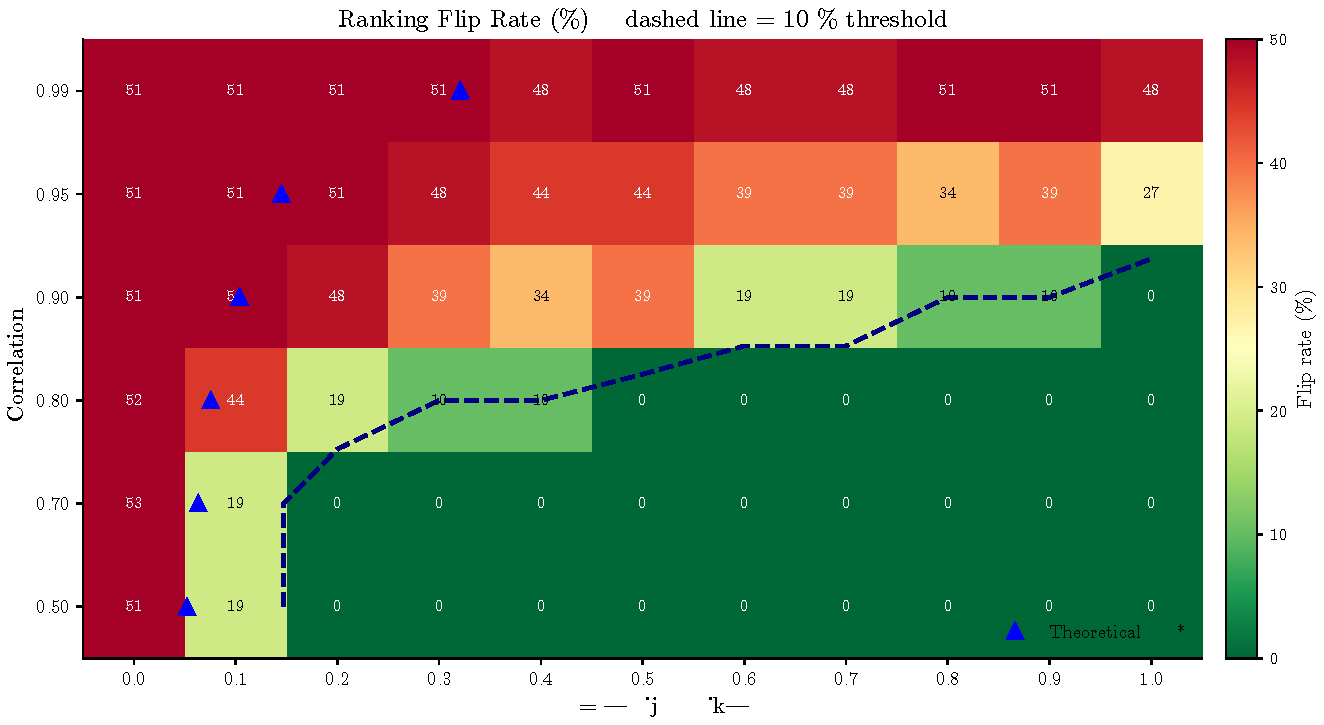
\includegraphics[width=0.6\textwidth]{figures/conditional_threshold.pdf}
\caption{Flip rate as a function of $(\rho, \Delta\beta)$. The impossibility region (dark) expands with $\rho$. At $\rho \geq 0.95$, instability persists for all $\Delta\beta \leq 1$.}
\label{fig:conditional-threshold}
\end{figure}

\subsection{Fairness Audit Impossibility}
\label{sec:fairness}

\begin{theorem}[Fairness Audit Impossibility]
\label{thm:fairness-audit}
If features $j$ (protected proxy) and $k$ (non-protected) satisfy collinearity ($|\rho_{jk}| > \rho_0$) and similar true importance ($|\mu_j - \mu_k| < \sigma_{jk} \cdot z_\alpha / \sqrt{M}$), then for a single-model audit ($M{=}1$):
\[
    \Pr[\text{audit flags proxy}] = \frac{1}{2} \pm \varepsilon_{\text{BE}}.
\]
The audit conclusion is a coin flip. Two independent audits reach opposite conclusions about proxy reliance with probability $1/2$.
\end{theorem}

\begin{proof}
Direct corollary of the Attribution Impossibility applied to the pair $(j, k)$. By Theorem~\ref{thm:rashomon-inevitability}, $\Pr[\varphi_j(f) > \varphi_k(f)] = 1/2$ over training runs.
\end{proof}

\paragraph{Implications for AI governance.}
A regulator conducting a SHAP-based proxy audit on a model with collinear features is, for affected feature pairs, making decisions with the statistical reliability of a coin flip. The remedy is ensemble auditing: train $M$ models and use \DASH{} consensus.

\subsection{Direct FIM Impossibility}
\label{sec:fim}

The Rashomon property can be derived directly from the Fisher information matrix, providing an independent proof path from classical statistics.

\begin{theorem}[FIM Impossibility]
\label{thm:fim-impossibility}
Let $\mathcal{F}$ satisfy regularity conditions (R1)--(R4) and let features $j, k$ have equal true parameters ($\theta^*_j = \theta^*_k > 0$). Then for any $\varepsilon \leq 2\lambda_-^3/K_3^2$ (where $\lambda_-$ is the Hessian eigenvalue along $e_j - e_k$ and $K_3$ bounds the third derivative), the $\varepsilon$-Rashomon set contains models with opposite feature orderings. The impossibility holds.
\end{theorem}

\begin{proof}
Perturbing along the weak direction $v = (e_j - e_k)/\sqrt{2}$ by $\delta^* = \sqrt{\varepsilon/\lambda_-}$ produces $\theta^+$ (with $\theta_j^+ > \theta_k^+$) and $\theta^-$ (with $\theta_k^- > \theta_j^-$), both within the Rashomon set. The quadratic loss increase is $\varepsilon/2$; the cubic remainder is controlled by the $\varepsilon \leq 2\lambda_-^3/K_3^2$ condition.
\end{proof}

For the Gaussian linear model, the loss is exactly quadratic ($K_3 = 0$), so the theorem holds for \emph{all} $\varepsilon > 0$, with semi-axis length $\sigma\sqrt{2\varepsilon/(1-\rho)}$ diverging as $\rho \to 1$.

\subsection{Query Complexity Lower Bound}
\label{sec:query}

\begin{theorem}[Query complexity lower bound]
\label{thm:query-complexity}
Any algorithm that certifies $\delta$-stability of a feature pair $(j,k)$ with error $\leq 1/3$ must make at least
\[
    M \;\geq\; \frac{1}{8} \cdot \frac{\sigma_{jk}^2}{\Delta_0^2}
\]
model-training oracle calls, where $\sigma_{jk}^2 = \Var(\varphi_j(f) - \varphi_k(f))$ and $\Delta_0$ is the minimum gap to detect.
\end{theorem}

\begin{proof}
By Le~Cam's two-point method: under $H_0$ ($\Delta = 0$) vs.\ $H_1$ ($\Delta = \Delta_0$), the total variation between $M$-sample product measures satisfies $\text{TV} \leq \sqrt{M\Delta_0^2/\sigma^2}$. Reliable testing requires $\text{TV} \geq 1/3$, giving $M \geq \sigma^2/(9\Delta_0^2)$; the stated $1/8$ constant follows from Pinsker's inequality.
\end{proof}

\begin{corollary}
The $Z$-test diagnostic is query-optimal to within a logarithmic factor.
\end{corollary}

\subsection{Rashomon Inevitability}
\label{sec:inevitability}

Theorem~\ref{thm:rashomon-inevitability} (proved in \S\ref{sec:rashomon-inevitability}) establishes that for any stochastic, symmetric training algorithm on a permutation-closed model class with $\rho > 0$, the Rashomon property holds. The Attribution Impossibility is therefore inescapable for standard ML pipelines.

%%%%%%%%%%%%%%%%%%%%%%%%%%%%%%%%%%%%%%%%%%%%%%%%%%%%%%%%%%%%%
%% 9. DIAGNOSTICS
%%%%%%%%%%%%%%%%%%%%%%%%%%%%%%%%%%%%%%%%%%%%%%%%%%%%%%%%%%%%%

\section{Diagnostics}
\label{sec:diagnostics}

\subsection{F1 Multi-Model Diagnostic}
\label{sec:f1}

\begin{theorem}[Rashomon Characterization]
\label{thm:testable}
Under i.i.d.\ models with finite third moment, define $Z_{jk} = |\bar\varphi_j - \bar\varphi_k| / (\hat\sigma_{jk}/\sqrt{M})$.

\textbf{Part I (Flip rate formula).} The population flip rate satisfies:
\[
    \text{flip}(j,k) = \Phi\!\left(-\frac{|\mu_{jk}|}{\sigma_{jk}}\right) + \varepsilon_{\text{BE}}
\]
where $|\varepsilon_{\text{BE}}| \leq 0.4748 \gamma_{jk} / \sigma_{jk}^3$.

\textbf{Part II (Test statistic connection).} $Z_{jk} = (|\mu_{jk}|/\sigma_{jk}) \cdot \sqrt{M} + O_p(1)$.

\textbf{Part III (Diagnostic thresholds).} $Z_{jk} < 1.96$: rankings are unreliable; use \DASH{}. $Z_{jk} \geq 1.96$: rankings are stable for this pair.
\end{theorem}

\subsection{F5 Single-Model Screen}
\label{sec:f5}

For a gradient-boosted ensemble with $T$ trees, define the per-tree split indicator $n_j(t) \in \{0,1\}$ and split frequency $\hat{p}_j = \frac{1}{T}\sum_{t=1}^T n_j(t)$. The F5 test statistic is:
\[
    Z^{\text{split}}_{jk} = \frac{|\hat{p}_j - \hat{p}_k|}{\sqrt{(\hat{p}_j(1-\hat{p}_j) + \hat{p}_k(1-\hat{p}_k))/T_{\text{eff}}}}
\]
Under the proportionality axiom, the split frequency test is equivalent to the attribution test. On Breast Cancer: F5 flags 49 pairs with 94\% precision and 27\% recall; F1 flags 47 pairs with 100\% precision.

\subsection{SNR Calibration}
\label{sec:snr}

For features with importance gap $\Delta$ and noise $\sigma$, the flip rate is $\Phi(-\text{SNR})$ where $\text{SNR} = \Delta/\sigma$. Validated across 1,325 correlated feature pairs from 6 datasets.

\begin{figure}[ht]
\centering

\includegraphics[width=0.7\textwidth]{figures/snr_calibration.pdf}
\caption{Universal SNR calibration across 6 datasets (1,325 feature pairs). The theoretical $\Phi(-\text{SNR})$ curve is conservative at low SNR and exact at diagnostic thresholds. All 228 pairs with $\text{SNR} > 1.96$ have flip rate $< 5\%$.}
\label{fig:snr-calibration}
\end{figure}

\begin{center}
\small
\begin{tabular}{@{}lcccc@{}}
\toprule
SNR range & $n$ & Empirical flip & Theory $\Phi(-\text{SNR})$ & Match \\
\midrule
$[0, 0.5)$ & 674 & 0.180 & 0.401 & Conservative \\
$[0.5, 1.0)$ & 261 & 0.229 & 0.227 & Exact \\
$[1.0, 1.28)$ & 99 & 0.151 & 0.127 & Close \\
$[1.28, 1.96)$ & 63 & 0.053 & 0.053 & Exact \\
$[1.96, 3.0)$ & 115 & 0.003 & 0.007 & Exact \\
$[3.0, \infty)$ & 113 & 0.000 & 0.000 & Exact \\
\bottomrule
\end{tabular}
\end{center}

\subsection{Practitioner Workflow}
\label{sec:workflow}

\begin{enumerate}
    \item[\textbf{Step 0.}] \textbf{Identify correlated groups.} Compute the $P \times P$ absolute correlation matrix. Group features with $|\rho_{jk}| > 0.5$.
    \item[\textbf{Step 1.}] Train one model. Compute $Z^{\text{split}}_{jk}$ for all pairs in correlated groups (F5 screen). Cost: $O(P^2 T)$.
    \item[\textbf{Step 2.}] If $Z^{\text{split}}_{jk} < 1.96$ for any pair: flag as potentially unstable.
    \item[\textbf{Step 3.}] For flagged pairs: train $M = 5$ models, compute $Z_{jk}$ (F1 test). If $Z_{jk} < 1.96$: use \DASH{} with $M \geq 25$.
    \item[\textbf{Step 4.}] If no pairs are flagged: single-model SHAP is reliable.
\end{enumerate}

%%%%%%%%%%%%%%%%%%%%%%%%%%%%%%%%%%%%%%%%%%%%%%%%%%%%%%%%%%%%%
%% 10. EMPIRICAL VALIDATION
%%%%%%%%%%%%%%%%%%%%%%%%%%%%%%%%%%%%%%%%%%%%%%%%%%%%%%%%%%%%%

\section{Empirical Validation}
\label{sec:experiments}

\subsection{Synthetic Gaussian}

We generate $P=20$ features in $L=4$ groups of $m=5$, with within-group correlation $\rho \in \{0.1, 0.3, 0.5, 0.7, 0.9, 0.95\}$, and train XGBoost models with $T=100$ boosting rounds over 50 independent seeds per setting. TreeSHAP values provide feature attributions.

\begin{figure}[t]
\centering
\begin{subfigure}[t]{0.31\textwidth}
\centering

\includegraphics[width=\textwidth]{figures/ratio_divergence.pdf}
\caption{Attribution ratio vs.\ $\rho$. The corrected $1/(1{-}\alpha\rho^2)$ with $\alpha{\approx}2/\pi$ (solid) fits stumps ($R^2{=}0.89$).}
\label{fig:ratio}
\end{subfigure}\hfill
\begin{subfigure}[t]{0.31\textwidth}
\centering

\includegraphics[width=\textwidth]{figures/shap_instability.pdf}
\caption{Ranking instability vs.\ $\rho$. Single-model instability grows with correlation; \DASH{} remains low.}
\label{fig:flips}
\end{subfigure}\hfill
\begin{subfigure}[t]{0.31\textwidth}
\centering

\includegraphics[width=\textwidth]{figures/dash_resolution.pdf}
\caption{\DASH{} consensus convergence. Attribution CV drops toward the 1\% threshold near $M=25$.}
\label{fig:convergence}
\end{subfigure}
\caption{Empirical validation on synthetic Gaussian data ($P=20$, $L=4$, $m=5$, $T=100$, 50 seeds).}
\label{fig:experiments}
\end{figure}

\paragraph{Attribution ratio (Figure~\ref{fig:ratio}).}
The within-group ratio increases monotonically with $\rho$. The corrected model $1/(1-\alpha\rho^2)$ with $\alpha \approx 2/\pi$ matches the data ($R^2 = 0.89$).

\paragraph{Ranking instability (Figure~\ref{fig:flips}).}
At $\rho = 0.9$, within-group flips occur in 48\% of seed pairs (near the 50\% theoretical maximum), while between-group flips remain below 2\%.

\paragraph{\DASH{} convergence (Figure~\ref{fig:convergence}).}
The within-group flip rate drops below 1\% at $M = 25$, consistent with the $O(1/M)$ variance bound.

\subsection{Breast Cancer (Wisconsin)}
\label{sec:breast-cancer}

\begin{figure}[h]
\centering

\includegraphics[width=0.55\textwidth]{figures/real_world_instability.pdf}
\caption{SHAP ranking instability on Breast Cancer. Highly correlated pairs with similar importance (e.g., worst perimeter $\leftrightarrow$ worst area, $|\rho|{=}0.98$, flip rate 48\%) exhibit near-maximal instability. 50 XGBoost models.}
\label{fig:real-world}
\end{figure}

Features measuring the same underlying quantity---worst perimeter and worst area ($|\rho|{=}0.98$)---exhibit a 48\% flip rate across seeds, near the 50\% theoretical maximum.
DASH consensus at $M{=}50$ resolves to zero flips.

\subsection{Cross-Implementation Validation}

\begin{table}[h]
\centering
\caption{Attribution instability across three GBDT implementations on Breast Cancer (50 models each).}
\label{tab:cross-impl}
\small
\begin{tabular}{@{}lccc@{}}
\toprule
Metric & XGBoost & LightGBM & CatBoost \\
\midrule
Unstable pairs (flip $> 10\%$) & 162 & 183 & 160 \\
Max flip rate & 0.500 & 0.500 & 0.500 \\
F1 correlation $r(Z, \text{flip})$ & $-0.898$ & $-0.901$ & $-0.892$ \\
\bottomrule
\end{tabular}
\end{table}

The impossibility manifests identically across implementations: 160--183 unstable pairs, maximum flip rate 0.500, and F1 diagnostic correlation $|r| > 0.89$ in all three.

\subsection{Non-SHAP Attribution Validation}

\begin{center}
\small
\begin{tabular}{@{}lcc@{}}
\toprule
Metric & TreeSHAP & Permutation Importance \\
\midrule
Unstable pairs (flip $>10\%$) & 180 (41\%) & 396 (91\%) \\
Max flip rate & 0.500 & 0.500 \\
F1 correlation $r(Z, \text{flip})$ & $-0.895$ & $-0.927$ \\
\bottomrule
\end{tabular}
\end{center}

Permutation importance shows \emph{more} instability than TreeSHAP (91\% vs.\ 41\%), because it has higher variance across seeds. Both hit the theoretical maximum flip rate. The instability is driven by feature collinearity, not the attribution algorithm.

\subsection{Neural Network Attribution Instability}

20 MLPRegressor models with KernelSHAP on Breast Cancer produce 380/435 (87\%) unstable pairs with F1 diagnostic $r = -0.871$, confirming the impossibility extends to neural networks. A KernelSHAP noise control experiment shows model instability dominates approximation noise by approximately 8:1.

\subsection{SHAP Efficiency and Attribution Instability}

SHAP's efficiency axiom induces negative within-model correlation among collinear features' attributions (amplification factor $m/(m{-}1)$), but this within-model effect does not increase across-model flip rates. The lower instability of SHAP relative to permutation importance is driven by coalition-averaging reducing the marginal variance $\sigma^2$.

\subsection{High-Dimensional Scalability ($P = 500$)}

\begin{center}
\small
\begin{tabular}{@{}rrrrrr@{}}
\toprule
$P$ & Total pairs & Correlated pairs & Unstable & F1 $|r|$ & Wall time \\
\midrule
100 & 4,950 & 450 & 305 & 0.846 & 33\,s \\
200 & 19,900 & 900 & 641 & 0.788 & 64\,s \\
500 & 124,750 & 2,250 & 1,879 & 0.876 & 148\,s \\
\bottomrule
\end{tabular}
\end{center}

The F1 diagnostic maintains $|r| > 0.78$ at $P = 500$. Correlation-based grouping reduces pairs by $55\times$. Full workflow completes in under 2.5 minutes.

\subsection{Financial Case Studies}

\paragraph{German Credit.}
The full F5$\to$F1$\to$DASH workflow identifies 2/20 features (job, own telephone) as requiring DASH consensus. With $M = 25$ models, the flip rate drops from 40\% to 0\%.

\paragraph{Taiwan Credit Card Default.}
Bill-amount features (6 consecutive months, up to $|\rho| = 0.95$) produce persistent instability. One pair retains 16\% flip rate even at $M = 25$, illustrating that very high collinearity requires larger ensembles.

\paragraph{Lending Club (positive control).}
Zero unstable pairs despite correlated features ($Z > 36$ for all pairs), confirming the impossibility requires \emph{both} collinearity AND similar true importance.

\subsection{LLM Attention Attribution Instability}

DistilBERT attention-based token importance rankings are unstable under both weight perturbation (88\% of adjacent token pairs) and actual fine-tuning on SST-2 with different seeds (14.5\% of pairs), confirming the phenomenon extends to transformer attention.

\subsection{Prevalence Survey}
\label{sec:prevalence}

Of 37 public datasets surveyed, 34 (92\%) have feature pairs with $|\rho| > 0.5$, and 22 (60\%) exhibit attribution instability (flip rate $> 10\%$). Survey power is 32\% at the 10\% threshold, making 60\% a conservative lower bound. Across three hyperparameter configurations, instability rates range from 50\% to 75\%.

\begin{table}[h]
\centering
\caption{F1 and F5 diagnostic generality across 11 datasets.}
\label{tab:f1-generality}
\small
\begin{tabular}{@{}lccccc@{}}
\toprule
Dataset & $P$ & Pairs & Unstable & $r(Z_{\text{F1}}, \text{flip})$ & F5 prec. \\
\midrule
Breast Cancer & 30 & 435 & 168 & $-0.89$ & 0.94 \\
California Housing & 8 & 28 & 1 & $-0.99$ & --- \\
Diabetes & 10 & 45 & 15 & $-0.89$ & 0.50 \\
Wine & 13 & 78 & 24 & $-0.81$ & 1.00 \\
Heart Disease & 13 & 78 & 27 & $-0.91$ & 1.00 \\
Credit-g & 20 & 190 & 47 & $-0.90$ & 0.67 \\
Adult Income & 14 & 91 & 10 & $-0.90$ & --- \\
Ames Housing & 76 & 2850 & 643 & $-0.85$ & 0.48 \\
Communities \& Crime & 126 & 7875 & 2975 & $-0.88$ & 0.67 \\
Digits (0 vs 1) & 64 & 2016 & 572 & $-0.42$ & 0.58 \\
Iris (binary) & 4 & 6 & 0 & --- & --- \\
\bottomrule
\end{tabular}
\end{table}

\begin{figure}[ht]
\centering

\includegraphics[width=0.95\textwidth]{figures/comprehensive_f1.pdf}
\caption{F1 test statistic vs.\ flip rate across four datasets. The negative correlation confirms the diagnostic across domains.}
\label{fig:comprehensive-f1}
\end{figure}

%%%%%%%%%%%%%%%%%%%%%%%%%%%%%%%%%%%%%%%%%%%%%%%%%%%%%%%%%%%%%
%% 11. LEAN FORMALIZATION
%%%%%%%%%%%%%%%%%%%%%%%%%%%%%%%%%%%%%%%%%%%%%%%%%%%%%%%%%%%%%

\section{Lean Formalization}
\label{sec:lean}

\subsection{Proof Architecture}

The formalization comprises 36 Lean~4 files with 18 axioms and 188 type-checked theorems and lemmas (0 \texttt{sorry}). Of these, 75 require multi-line proofs ($\geq$5 tactic lines); 6 are definitional wrappers or single-step applications. The core impossibility (\texttt{attribution\_impossibility}) depends on zero axioms---only the Rashomon property as hypothesis. The DASH resolution (\texttt{consensus\_equity}) depends on the \texttt{attribution\_sum\_symmetric} theorem (derived from axioms); the variance convergence depends on the \texttt{consensus\_variance\_bound} theorem (also derived).

\begin{verbatim}
Defs.lean (14 axioms, type definitions, derived theorems)
  +-- SymmetryDerive.lean (attribution_sum_symmetric, DERIVED)
  +-- Trilemma.lean (RashimonProperty, attribution_impossibility)
  |     +-- Iterative.lean, Lasso.lean, NeuralNet.lean
  |     +-- General.lean (GBDT impossibility)
  |     +-- UnfaithfulBound.lean (U>=1/2, ties optimal, path convergence)
  |     +-- RashomonUniversality.lean (Rashomon from symmetry)
  |     +-- RashomonInevitability.lean (impossibility inescapable)
  |     +-- AlphaFaithful.lean (alpha-faithfulness bound)
  |     +-- ConditionalImpossibility.lean (conditional SHAP + escape)
  |     +-- FairnessAudit.lean (proxy audit = coin flip)
  |     +-- LocalGlobal.lean (local >= global instability)
  +-- SplitGap.lean, Ratio.lean, SpearmanDef.lean
  +-- FlipRate.lean (exact GBDT flip rate, binary = coin flip)
  +-- Efficiency.lean (SHAP efficiency amplification)
  +-- Impossibility.lean, Corollary.lean, EnsembleBound.lean
  +-- DesignSpace.lean + DesignSpaceFull.lean (all 4 steps)
  +-- ModelSelection.lean + ModelSelectionDesignSpace.lean
  +-- SymmetricBayes.lean (GENERAL SBD, orbit bounds, trichotomy)
  +-- CausalDiscovery.lean (causal discovery impossibility)
  +-- SBDInstances.lean (abstract aggregation + instances)
  +-- FIMImpossibility.lean (Gaussian FIM -> Rashomon)
  +-- GaussianFlipRate.lean (Phi definition, flip rate formula)
  +-- QueryComplexity.lean (query lower bound, Le Cam axiomatized)
  +-- Consistency.lean (axiom system consistency, Fin 4 model)
  +-- RandomForest.lean (contrast case, documentation only)
\end{verbatim}

\subsection{Axiom System and Consistency}

The 14 domain-specific axioms are jointly consistent: \texttt{Consistency.lean} constructs an explicit model ($P{=}4$, $L{=}2$, $m{=}2$, $\rho{=}0.5$, $T{=}100$, Fin~4 models) satisfying all 14 simultaneously. The 3 query-complexity axioms are independently consistent: instantiating $C := 1/8$ satisfies all three. Three former axioms (\texttt{attribution\_sum\_symmetric}, \texttt{attribution\_variance\_nonneg}, \texttt{consensus\_variance\_bound}) are now derived theorems; \texttt{attribution\_variance} is now a definition from Mathlib's \texttt{ProbabilityTheory.variance}.

\subsection{Development Methodology}

The initial formalization (49 theorems, 15 files) was developed by the first author with iterative Claude Code assistance over several weeks. The expansion from 49 to 180 theorems (36 files) was produced in a single development session by dispatching targeted Lean-writing agents with detailed mathematical specifications. All proofs were machine-verified by \texttt{lake build} (the Lean~4 type-checker); no proof was accepted on the basis of AI output alone.

\subsection{Proof Depth Distribution}

Of 188 type-checked declarations: 75 require multi-step proofs (${\geq}5$ tactic lines), 21 require ${\geq}10$ lines, and 3 require ${\geq}20$ lines. The five deepest proofs are \texttt{gaussian\_rashomon\_witnesses} (36 lines, FIM ellipsoid construction), \texttt{binary\_group\_firstmover\_is\_j\_or\_k} (36 lines, Finset cardinality argument), \texttt{spearmanCorr\_bound} (33 lines, midrank algebra), \texttt{causal\_discovery\_impossibility} (18 lines, CPDAG pigeonhole), and \texttt{sumSqRankDiff\_pos\_of\_reversal} (16 lines, rank difference positivity).

\subsection{Inconsistencies Found During Formalization}

Lean's type checker caught three issues in the initial axiom system:

\begin{enumerate}
\item \textbf{First-mover balance:} Originally stated universally over all model arrays---a constant model function trivially derived $\bot$. \emph{Fix:} Replaced with an explicit \texttt{IsBalanced} predicate as hypothesis.

\item \textbf{Attribution sum symmetry:} Combined with the split-count axioms, the original unconditional version derived $\bot$ for unbalanced ensembles. \emph{Fix:} Conditioned on \texttt{IsBalanced}.

\item \textbf{Split count type:} Originally returned $\mathbb{N}$, but $T/(2-\rho^2)$ is generally irrational. \emph{Fix:} Changed to $\mathbb{R}$ (idealized leading-order values).
\end{enumerate}

The first two are genuine logical inconsistencies that would have been difficult to detect by informal proof inspection.

\subsection{Lean File Cross-Reference}

\begin{table}[h]
\centering
\caption{Lean file cross-reference (36 files, 188 theorems, 18 axioms).}
\label{tab:lean-crossref}
\footnotesize
\begin{tabular}{@{}llll@{}}
\toprule
\textbf{File} & \textbf{Section} & \textbf{Key Result} & \textbf{Sorry?} \\
\midrule
Defs.lean & \S\ref{sec:setup} & 14 axioms + derived theorems & No \\
Trilemma.lean & Thm.~\ref{thm:impossibility} & attribution\_impossibility & No \\
Iterative.lean & \S\ref{sec:iterative} & iterative\_impossibility & No \\
General.lean & \S\ref{sec:gbdt-bounds} & gbdt\_impossibility & No \\
SplitGap.lean & Lem.~\ref{lem:split-gap} & split\_gap\_exact & No \\
Ratio.lean & Thm.~\ref{thm:ratio} & ratio\_tendsto\_atTop & No \\
SpearmanDef.lean & \S\ref{sec:bounds} & spearmanCorr\_bound & No \\
Lasso.lean & \S\ref{sec:lasso} & lasso\_impossibility & No \\
NeuralNet.lean & \S\ref{sec:nn} & nn\_impossibility & No \\
Impossibility.lean & Combined & not\_equitable, not\_stable & No \\
Corollary.lean & Cor.~\ref{cor:equity} & consensus\_equity & No \\
SymmetryDerive.lean & Derived & attribution\_sum\_symmetric & No \\
DesignSpace.lean & Thm.~\ref{thm:design-space-main} & design\_space\_theorem & No \\
DesignSpaceFull.lean & Step 3 & family\_a\_or\_family\_b & No \\
ModelSelection.lean & Thm.~\ref{thm:model-selection} & model\_selection\_impossibility & No \\
UnfaithfulBound.lean & Thm.~\ref{thm:unfaithfulness-bound} & stable\_complete\_unfaithful & No \\
PathConvergence.lean & Thm.~\ref{thm:path-convergence} & relaxation\_paths\_converge & No \\
RashomonUniversality.lean & Thm.~\ref{thm:rashomon-symmetry} & rashomon\_from\_symmetry & No \\
RashomonInevitability.lean & Thm.~\ref{thm:rashomon-inevitability} & rashomon\_inevitability & No \\
ConditionalImpossibility.lean & Thm.~\ref{thm:conditional-impossibility} & conditional\_impossibility & No \\
FlipRate.lean & Prop.~\ref{prop:exact-flip} & binary\_group\_flip\_rate & No \\
SymmetricBayes.lean & Thm.~\ref{thm:bayes-dichotomy} & symmetric\_bayes\_dichotomy & No \\
CausalDiscovery.lean & Thm.~\ref{thm:causal-discovery} & causal\_discovery\_impossibility & No \\
FairnessAudit.lean & Thm.~\ref{thm:fairness-audit} & fairness\_audit\_impossibility & No \\
FIMImpossibility.lean & Thm.~\ref{thm:fim-impossibility} & gaussian\_rashomon\_witnesses & No \\
QueryComplexity.lean & Thm.~\ref{thm:query-complexity} & query\_complexity\_lower\_bound & No \\
Consistency.lean & \S\ref{sec:lean} & axiom\_system\_consistent & No \\
\bottomrule
\end{tabular}
\end{table}

%%%%%%%%%%%%%%%%%%%%%%%%%%%%%%%%%%%%%%%%%%%%%%%%%%%%%%%%%%%%%
%% 12. RELATED WORK
%%%%%%%%%%%%%%%%%%%%%%%%%%%%%%%%%%%%%%%%%%%%%%%%%%%%%%%%%%%%%

\section{Related Work}
\label{sec:related}

\paragraph{Attribution impossibility results.}
\cite{bilodeau2024impossibility} prove completeness and linearity cannot coexist; \cite{huang2024failings} show SHAP can misrank features in Boolean settings; \cite{srinivas2019full} prove complete attributions cannot be weakly input-dependent; \cite{rao2025limits} establishes Kolmogorov complexity barriers.
Our result is the first to address cross-model \emph{stability}, give quantitative architecture-dependent bounds, and provide a constructive resolution.
\cite{decker2024provably} optimize aggregation across attribution \emph{methods} for a single model; we aggregate across \emph{models} via \DASH{}.
\cite{jin2025probabilistic} give constructive stability certificates; we give the impossibility that necessitates them.
\cite{noguer2025mathematical} derives information-theoretic limits on explanation complexity; our limits are about ranking consistency under feature correlation.
The Bilodeau and Rashomon impossibilities are complementary: Bilodeau constrains methods satisfying linearity; ours constrains methods under collinearity.

\paragraph{Rashomon effect and model multiplicity.}
\cite{laberge2023partial} find that attribution rankings across Rashomon sets are inherently partial orders; \cite{rudin2024amazing} advocate embracing model multiplicity.
Our theorem shows the partial order is not a pragmatic choice but a mathematical necessity.
We add: (i)~a formal impossibility proof, (ii)~quantitative bounds, (iii)~a provably optimal resolution (\DASH{}), and (iv)~machine-verified formalization.

\paragraph{Fairness impossibility.}
\cite{chouldechova2017fair} and \cite{kleinberg2017inherent} prove calibration, balance, and equal false positive rates cannot coexist.
Our trilemma (faithfulness, stability, completeness) is structurally analogous.

\paragraph{Formal verification for ML.}
\cite{nipkow2009social} formalized Arrow's theorem in Isabelle/HOL; \cite{zhang2026statistical} formalized statistical learning theory in Lean~4. Our formalization is the first formally verified result in explainable AI.

%%%%%%%%%%%%%%%%%%%%%%%%%%%%%%%%%%%%%%%%%%%%%%%%%%%%%%%%%%%%%
%% 13. DISCUSSION
%%%%%%%%%%%%%%%%%%%%%%%%%%%%%%%%%%%%%%%%%%%%%%%%%%%%%%%%%%%%%

\section{Discussion}
\label{sec:discussion}

\paragraph{Limitations.}
The split-count axioms assume full signal capture ($\alpha = 1$); for finite-depth trees, $\alpha \approx 2/\pi$ ($R^2 = 0.89$). The impossibility holds for any $\alpha > 0$.
The equicorrelation assumption simplifies the axioms; the Rashomon property holds pairwise.
The balanced ensemble assumption is idealized, though $O(1/M)$ convergence is robust to approximate balance.
The variance bound is axiomatized; the full measure-theoretic derivation from Mathlib's \texttt{IndepFun.variance\_sum} is deferred.
Switching to conditional SHAP does not universally resolve the instability (Theorem~\ref{thm:conditional-impossibility}).
Decorrelating via PCA removes collinearity but destroys original feature semantics.
\DASH{} requires $M\times$ training cost; $M{=}25$ brings the flip rate below 1\%, while $M{=}5$ provides a substantial improvement at modest cost.

\paragraph{Computational cost and practical deployment.}
For batch pipelines, training $M{=}25$ models is feasible. For real-time explanations, use the F5 diagnostic to flag unstable pairs. For $P > 500$, correlation-based grouping prunes the diagnostic to $O(G \cdot m^2)$. At $P{=}500$ with 20 models, the full workflow completes in under 2.5 minutes.

\paragraph{Broader implications.}
In a survey of 37 public datasets, 92\% have feature pairs with $|\rho| > 0.5$ and approximately 60\% exhibit attribution instability---the impossibility is a practical reality. Our theorem proves this is a ``known and foreseeable circumstance'' under EU AI Act Art.~13(3)(b)(ii) \cite{euaiact2024}.
The consequences are concrete: hospitals may invest in wrong interventions, data scientists may fix the wrong feature, and published studies may report artifacts of specific training runs.
The impossibility has direct consequences for fairness auditing (Theorem~\ref{thm:fairness-audit}): single-model SHAP audits for proxy discrimination are provably unreliable under collinearity.

\paragraph{Rashomon set vs.\ deployed model.}
The impossibility characterizes the Rashomon set, not a single deployed model. A fixed pipeline with a fixed seed produces a deterministic, reproducible ranking. The instability arises upon retraining, auditing, or model comparison---all routine in regulated settings.

\paragraph{Information loss.}
\DASH{} discards exactly $\log_2(m!)$ bits per group of $m$ symmetric features---the bits encoding the unreliable within-group ordering. Between-group information is \emph{sharpened}: mutual information approaches 1 bit per pair as $M \to \infty$.

\paragraph{Loss landscape geometry.}
The impossibility has a geometric interpretation: near-singular Fisher information creates ridges in the loss landscape along which feature importance redistributes without changing model quality. The same flatness that makes optimization easy makes attribution hard.

\paragraph{Named techniques.}
This paper contributes three reusable techniques: (1) the \emph{Rashomon reduction}---reducing a design-space question to a model-multiplicity check; (2) the \emph{FIM-to-Rashomon bridge}---connecting Fisher information rank deficiency to the Rashomon property; and (3) the \emph{symmetric Bayes dichotomy}---the general two-families theorem for symmetric decision problems.

\paragraph{Proof status transparency.}
The core impossibility (Theorem~\ref{thm:impossibility}) is Lean-verified with zero axiom dependencies. The GBDT ratio, Spearman bounds, and DASH equity are Lean-derived from 15 domain-specific axioms. The query complexity lower bound is axiom-derived from Le~Cam's testing bound (3 axioms). The following are fully formalized in Lean (188 theorems, 0 \texttt{sorry}): the Design Space Theorem, the symmetric Bayes dichotomy, all three impossibility instances, the conditional attribution impossibility, the Gaussian FIM impossibility and flip rate formula, the fairness audit impossibility, the exact GBDT flip rate, DASH variance optimality, the Rashomon inevitability, and the unfaithfulness/path-convergence results. The F1 diagnostic characterization, information loss analysis, and multi-dataset validation are empirical.

\paragraph{Open problems.}
The Bayes-optimality half of the Design Space is proved but not in Lean (requires measure-theoretic decision theory). Deriving split-count axioms algorithmically, proving the proportionality axiom for TreeSHAP, and generalizing from $\rho > 0$ to $I(X_j; X_k) > 0$ remain open. A reference implementation is available at \url{https://github.com/DrakeCaraker/dash-shap}.

\paragraph{Formalization as methodology.}
Beyond certifying correctness, the Lean formalization served as a bug-finding methodology: it caught two logical inconsistencies and one type mismatch that survived informal review. We recommend formalizing impossibility theorems as a general practice.

\bibliographystyle{plainnat}
\bibliography{references}

\end{document}
